\chapter{Experiments}
\section{Equipment}
\begin{itemize}
\item 750W Microwave oven
\item Bacon: two types, thick bacon (``skogsbacon'') and regular bacon.
\item Ruler
\item Slide caliper
\item Mettler AE50 (weight)
\item Paper
\item Grease-proof paper
\item Scissors
\end{itemize}

\section{Execution}

The bacon slice was laid between one sheet of paper on top, and one sheet of
grease-proof paper beneath. Earlier experiments with dual layer paper had
resulted in fusing of the bacon and paper. Still we needed to absorb the fat
output, so a compromise was to combine paper (for fat absorption) and
grease-proof paper (preventing fat spillage). $\\$

First the weight of the wrapping was measured (paper and grease-proof paper), and
then the dimensions of the bacon - weight, length, thickness and
width - were measured. The bacon slice was wrapped and baked in the microwave oven for the
desired amount of time. After completion new dimensions, both of
bacon and wrapping were measured, and number between 0.0-1.0 describing the
crispness of the bacon was assigned.

\section{Measurements}

First weight gain in the wrapping was measured, then the weight loss in the
bacon. It was assumed that all gain in the wrapping came from fat absorption, and that the
weight loss in the bacon consisted of fat melting and water evaporation. The new
dimensions of the bacon were also documented. $\\$

The assumptions combined with the measurements made it possible to quantify fat
loss, water loss and shrinkage of the bacon. All data was recorded onto data
sheets of the form \cref{fig:datasheet}, see \cref{avs:datasheet}. This gave the plots in
\cref{fig:thick_bacon} and \cref{fig:regular_bacon}.

\begin{figure}[ht!]
\subfloat[Thick
bacon]{\label{fig:thick_bacon}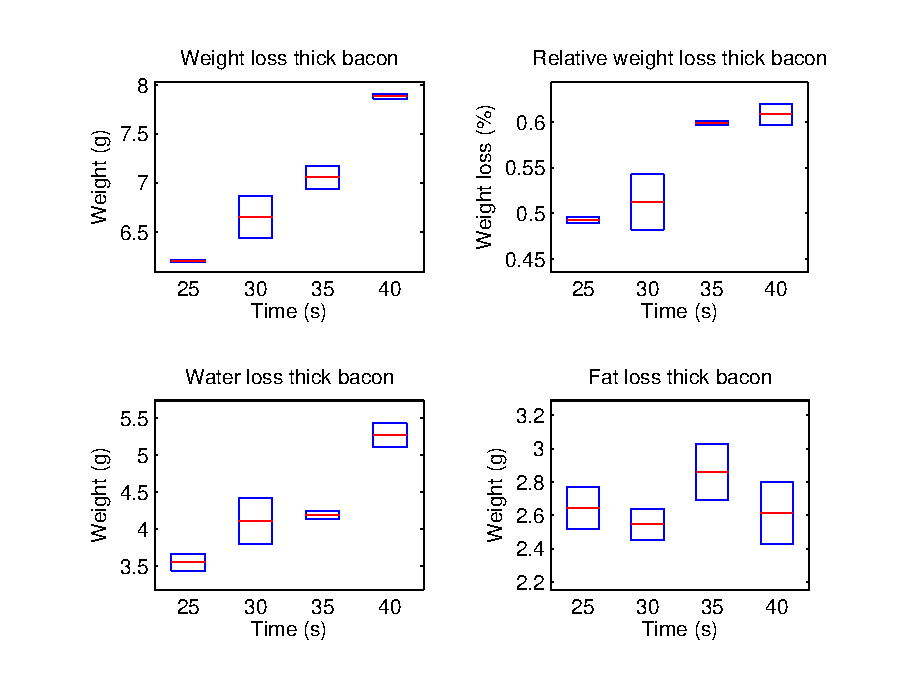
\includegraphics[width=0.5\textwidth]{thick_bacon}}\qquad
\subfloat[Regular bacon]{\label{fig:regular_bacon}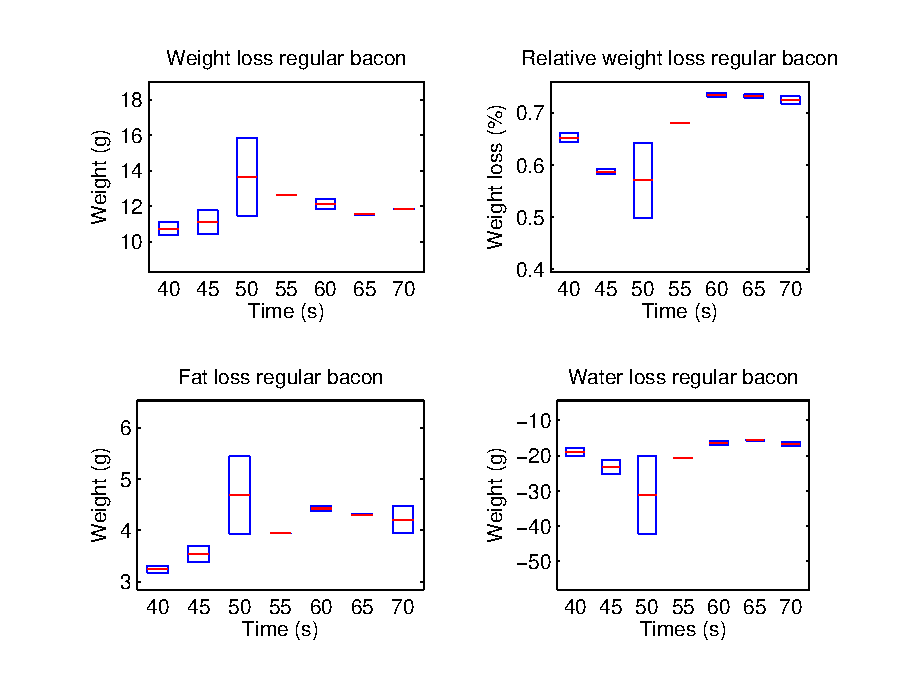
\includegraphics[width=0.5\textwidth]{regular_bacon}}
\caption{Schematic representation of measured data}
\label{fig:baconplot}
\end{figure}

\section{Results and discussion}

As can be seen in \cref{fig:thick_bacon} the water loss from 30-35 seconds is
approximately constant, while the fat loss is increasing on the same
time interval. This shows that around 30-35 seconds fat starts to melt,
``stealing'' heat from the water, this is in correspondence with weight loss as
a function of time. The fat loss continues to increase linearly
up to about 50 seconds, see \cref{fig:regular_bacon}. After 50
seconds the fat loss stabilizes, indicating that no more fat can be lost, and
that further baking time results in burnt bacon. $\\$

These results agree with expectations that the weight loss would
stabilize after a critical time, something that is clearly demonstrated in
\cref{fig:baconplot}. It is worth commenting that the big variation in
\cref{fig:regular_bacon} for $t = 50$s is due to one enormous (relative to the
others) bacon slice.

